\documentclass[11pt,openright,a4paper]{report}
%%
%% This document template assumes you will use pdflatex.  If you are using
%% latex and dvipdfm to translate to pdf, insert dvipdfm into the options.
%%

%%
%% Package includes to provide the basic style
%%
\usepackage{harvard}    % Uses harvard style referencing
\usepackage{graphicx}   % Permits import of various graphics formats
\usepackage{hyperref}   % Provides hyperlinks to sections automatically
\usepackage{pdflscape}  % Provides landscape mode for end code listings
\usepackage{multicol}   % Provides ability to split output into columns
\usepackage{listings}   % Provides styled code listings


%%
%% Set some page size changes from the standard article class
%%
\usepackage{calc}
\setlength{\parskip}{6pt}
\setlength{\parindent}{0pt}
\addtolength{\hoffset}{-0.5cm}
\addtolength{\textwidth}{2.5cm}


%%
%% Format definitions for the style
%%
\bibliographystyle{agsm}  %{alpha}
\citationstyle{dcu}
\pagestyle{headings}
\fussy


%%
%% Definitions to provide layout in the dissertation title pages
%%
\newenvironment{spaced}[1]
  {\begin{minipage}[c]{\textwidth}\vspace{#1}}
  {\end{minipage}}


\newenvironment{centrespaced}[2]
  {\begin{center}\begin{minipage}[c]{#1}\vspace{#2}}
  {\end{minipage}\end{center}}


\newcommand{\declaration}[2]{
  \thispagestyle{empty}
  \begin{spaced}{4em}
    \begin{center}
      \LARGE\textbf{#1}
    \end{center}
  \end{spaced}
  \begin{spaced}{3em}
    \begin{center}
      Submitted by: #2
    \end{center}
  \end{spaced}
  \begin{spaced}{5em}
    \section*{COPYRIGHT}

    Attention is drawn to the fact that copyright of this dissertation rests
    with its author. The Intellectual Property Rights of the products
    produced as part of the project belong to the author unless otherwise specified
    below, in accordance with the University of Bath's policy on intellectual property 
   (see http://www.bath.ac.uk/ordinances/22.pdf).

    This copy of the dissertation has been supplied on condition that anyone
    who consults it is understood to recognise that its copyright rests with its
    author and that no quotation from the dissertation and no information
    derived from it may be published without the prior written consent of
    the author.

    \section*{Declaration}
    This dissertation is submitted to the University of Bath in accordance
    with the requirements of the degree of Bachelor of Science in the
    Department of Computer Science. No portion of the work in this dissertation
    has been submitted in support of an application for any other degree
    or qualification of this or any other university or institution of learning.
    Except where specifically acknowledged, it is the work of the author.
  \end{spaced}

  \begin{spaced}{5em}
    Signed:
  \end{spaced}
  }


\newcommand{\consultation}[1]{%
\thispagestyle{empty}
\begin{centrespaced}{0.8\textwidth}{0.4\textheight}
\ifnum #1 = 0
This dissertation may be made available for consultation within the
University Library and may be photocopied or lent to other libraries
for the purposes of consultation.
\else
This dissertation may not be consulted, photocopied or lent to other
libraries without the permission of the author for #1 
\ifnum #1 = 1
year
\else
years
\fi
from the date of submission of the dissertation.
\fi
\vspace{4em}

Signed:
\end{centrespaced}
}

%%
%% END OF DEFINITIONS
%%

    %% These are the includes required for the doc 
\usepackage{url}
\usepackage{graphicx} 
\usepackage{booktabs}
\usepackage{float}
\title{High Performance Network Switch Solution Using Open Sourced Hardware}
\author{Zhouqiang Tu}
\date{MSc in Internet System and Security\\The University of Bath\\September 2016}


\begin{document}


% Set this to the language you want to use in your code listings (if any)
\lstset{language=Java,breaklines,breakatwhitespace,basicstyle=\small}


\setcounter{page}{0}
\pagenumbering{roman}


\maketitle
\newpage


% Set this to the number of years consultation prohibition, or 0 if no limit
\consultation{0}
\newpage


\declaration{High Performance Network Switch Solution Using Open Sourced Hardware}{Zhouqiang Tu}
\newpage


\abstract
The thesis introduces a solution to high performance network infrastructure reducing the latency significantly by using dual feeds. The hardware infrastructure implemented in the project is the open sourced hardware, different from the established commercial solutions. The major goal of the project is to prove that the cost in implementing ultra-low latency network can be reduced significantly by using the open sourced hardware, and assisted with FPGA. The project focuses on implementing the fat-tree network topology among three Raspberry Pi2 Model B with one Spartan FPGA, logically introducing the perfect shifting strategy in data intercommunication, implementing MPICH2 among three ARM CPUs, and infiniband RDMA memory accessing strategy to provide the scalability along with the MPI to the system. The experiments performed in the project shows that the solution reduces network latency significantly with reasonable cost in bandwidth and computational power. The system can be implemented in both high-frequency market data infrastructure and high-performance computational clusters as the distributed switch, for it meets the requirements of: low-latency data transmission, reliable end-to-end communication and acceleration in collective communication in MPI.  
\newpage

\tableofcontents
\newpage
\listoffigures
\newpage
\listoftables
\newpage

\setcounter{page}{1}
\pagenumbering{arabic}



\chapter{Thesis Background and Literature Review}
%% Uncomment this to include a separate tex file wih the introduction contents
\section{Thesis}
Financial instruments and organizations in the modern world needs to provide an live update on their current market status, and provide a package of information to its members and partners. The data they need to update is includes bid/ask prise, completed trades and other market status\cite{alexander2001market}. This package of information is aggregated, and streamed as 'Market Data Feed'. Modern financial market requires high performance infrastructure due to the implementation of automated trading system, which implements complicate market strategies and uses the data feed as sources\cite{le2009automated}. Modern strategies requires huge computational power to perform mathematical modelling, and high performance network to make the order ahead of any competitors.\\
Low latency infrastructure is invented to meet the market requirements, it is usually consisted of two parts,  computational nodes and network infrastructure. Existing solutions for the former part are customized servers, cloud computer farms and special data centres. They are programmed to perform data analysis over live market data feed, the outputs are trading behaviours packed as orders . Firms in computer network services are focusing on the latter part, as the latency in this part can be solved by engineering practises.\\
Solutions for low latency network usually come with high cost non-scalable hardware, and requires racks of server cabinets to install the devices. However, the entry barrier in the upfront investment for network infrastructure makes it difficult for medium or small financial institutions to start business in this field.\\
Researchers are looking forward to find alternative solutions to build network infrastructures that supports low latency market data feed. The researchers in high performance computation cluster provides a possible solution. The interconnect networks in supercomputers follows a different design in network interfaces. The improving design of parallel program architectural in supercomputers requires more efficient parallelism in network interface\cite{pang2014th}. We introduces the high scalable design and the fat-tree topology in the architecture into our design of high performance network switches, and achieve similar acceleration in data process as the existing commercial solutions.\\
\section{Objectives}
\subsection{Overall Design}
The project designed an experimental system over Raspberry Pi 2 Model B hardware, that supports 100Mbps Ethernet dual feeds as data source. The system should be flexible in error tolerance such as package loss, and scalable in implementing additional heterogeneous hardware. The network can be separated into two parts: the communication layer that supports low-latency network, and monitor system embedded in the SoC that implements additional features such as error tolerance. \\ 
The SoC system are interconnected as a homogeneous processing cluster. The task/thread management are performed by interconnected CPUs over multi-processor interfaces, memory solution for bandwidth requirement of high frequency data is RDMA protocols implemented over open sourced hardware memories. The FPGA attached in the master node is in charge of decoding, decompression and filtering for dual feeds.\\
\begin{figure}[htbp]
	\centering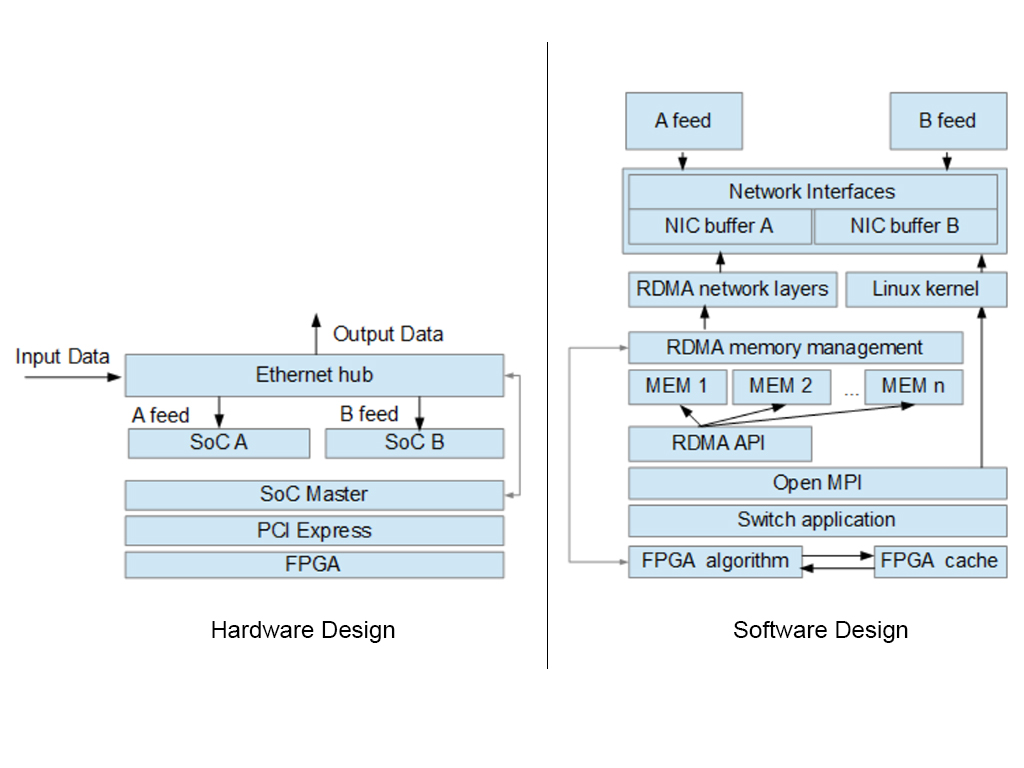
\includegraphics[width=3.5in]{picture/System_Design.jpg}
	\caption{System Design}
	\label{fig:system_design}
\end{figure}
This solution implements and improves the solution provided by the commercial firms in 10Gb Ethernet Switches, which introduces high performance computation chips to resolve the pressure in the network interface buffer. The improvement is in the layer of the high performance computing: in this solution, the HPC layer is not linked directly to the NIC in the board, but is interconnected by the Ethernet hub, which is much cheaper that 10Gb Ethernet switches. It sacrifices bandwidth in inner system to achieve similar efficiency in data processing by give spaces to heterogeneous scalable computational platforms, consisted by open sourced hardware like Raspberry Pi, and the fat-tree topology interconnection enables the cluster to expand without much cost.\\
The system can be implemented as the interconnection switch network for cloud computing clusters and high performance computer clusters. The design introduces the infrastructural solution for low-latency market data feed, utilizing data transmission efficiency with limited bandwidth, and the fat-tree topology network provides features in system monitoring and scalability in supporting massive computation.\\  
\subsection{Main Objective}
The main object for the project is to implement an experiment over a combined hardware-software environment with the features showing in table \ref{table:features}. The system is consisted of two parts:\\
\begin{itemize}
	\item The hardware part: creating physical connection among ARM based SoCs and FPGA accelerated data processor, and connect to the data feed via Ethernet cables;
	\item The software part: creating logical fat-tree topology network, that buffering dual feeds in the slave nodes and processing UDP packages via FPGA accelerated master node and other parallel user cores; 
\end{itemize}
\begin{table}[]
	\centering
	\caption{System Features}
	\label{table:features}
	\begin{tabular}{@{}l|l@{}}
		\toprule
		Features                                                                           & Description                                                                                                                                                                                                                                               \\ \midrule
		\begin{tabular}[c]{@{}l@{}}A-B data feed\\ handler\end{tabular}                    & \begin{tabular}[c]{@{}l@{}}The system needs to support dual data feed(A-B data feed)\\ to simulate the senario of ultra-low latency market data \\ transmission\end{tabular}                                                                              \\ \hline
		\begin{tabular}[c]{@{}l@{}}FPGA accelerated\\ UDP package processsing\end{tabular} & \begin{tabular}[c]{@{}l@{}}The decompression and filtering of dual UDP packages in \\ FPGA are proved to be more efficient than pure CPU \\ solutions, and can be expand to more general situations\\ in normal high frequency data networks\end{tabular} \\ \hline
		\begin{tabular}[c]{@{}l@{}}ARM based SoC \\ interconnection\end{tabular}           & \begin{tabular}[c]{@{}l@{}}Interconnection among ARM based SoC network makes it \\ possible to implement scalable buffer capacity and bandwidth\end{tabular}                                                                                              \\ \hline
		\begin{tabular}[c]{@{}l@{}}Fat tree \\ interconnect \\ network\end{tabular}        & \begin{tabular}[c]{@{}l@{}}Fat tree topology is proved to be efficient in \\ implementing interconnection network for massive parallel \\ computation, and flexible in scalable computational nodes.\end{tabular}                                         \\ \bottomrule
	\end{tabular}
\end{table}
\section{Literature review}
\subsection{Market Data Feed}
The principle of providing low latency market data feed is to provide users live data of current price information and trader status, including individual portfolio valuation, financial market data, trading activities and alarms, a matrix of these data forms an 'Order Book'. The data feeds have different price for varies delays, famous market data feed providers, or the data vendors, such as Yahoo finance, ThomsonReuters and Bloomberg provide combinations of pricing and other market information in different latencies. For example, data delayed over 5 minutes can be fetched from Yahoo finance API for free\cite{financeyahoo}, and ThomsonReuters provide paid services in different level of delay. Customers can choose to use designed data feed services to meet their business requirements, show in the reference to picture \ref{fig:1}.\\
\begin{figure}[htbp] 
\centering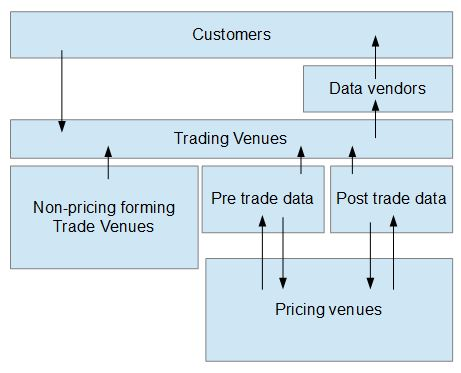
\includegraphics[width=3.5in]{picture/tradevenue.PNG} 
\caption{Relationship among trade venue, data vendors and customers}
\label{fig:1} 
\end{figure} 
\subsection{Low Latency Network Infrastructure}
Engineers provide solutions to achieve lower latency in network transmission for market data, including direct redundant fibre cables from trading centre to traders, shortest path transmission and dual data feed. For example, solution using microwave towers reducing the cost of digging tunnels for fibres and enabling signals transmit over the sphere is implemented between New Jersey and Chicago\cite{htfbackyard}, shows in the picture \ref{fig:2}. Engineers also developed 'dual-feed' mechanism to reduce the cost in retransmission when package lost\cite{zusman1999fault}.The introduction of dual feed, or the A-B feed of market data transmission uses two feeds with offset in delay to avoid significant failure such as delay or fault, especially for regional traders who want to trade across long geographical distances. \\

\begin{figure}[htbp]
\centering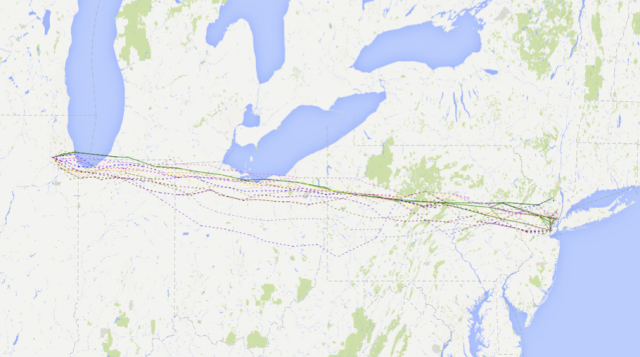
\includegraphics[width=3.5in]{picture/newyork-chicago.jpg}
\caption{Chicago-New Jersey microwave networks from data vendor Quincy Data}
\label{fig:2}
\end{figure}

\subsection{A-B Data Feed}
A-B feed structure requires two independent signals from one data provider, and the one feed(A) is several milliseconds faster than another feed(B). Relay stations between the sender and receiver need to decompress both feeds, filter and aggregate the package then transmit the data feed to the next station. Receiver also need a decompresser to handle the data from both feeds, reconstruct the original package and split the data into sub-streams forming process-specific subset of data, shows in picture \ref{fig:3}.\\
\begin{figure}[htbp]
	\centering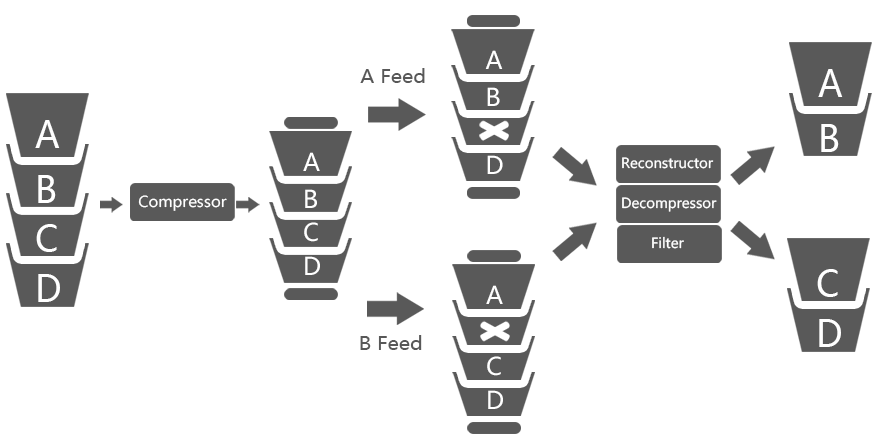
\includegraphics[width=3.5in]{picture/A-BFeed.PNG}
	\caption{Overview of A-B streaming infrastructure}
	\label{fig:3}
\end{figure}\\
Each data feed arrives in sequence with a prefixed header, containing information from abstracted layers of network protocols\cite{udpprotocol}. UDP protocol suggests UDP client to provide reliability services that the receiver should perform CRC check of the received package chains, and retransmit the chain if package lost found, timeout mechanism exacerbate the difficulty in providing low latency data service. A-B data feed reduces enable the rapid collect-dispatch system to provide output within 500 milliseconds\cite{zusman1999fault}.\\

\subsection{Scalable Interconnect Switches in Supercomputers}
Existing hardware solutions for low latency network is not suitable for mid sized institutions or individuals to start their usage of the network, and the development in building supercomputers provides an alternative solution to build infrastructure with equivalent function without implementing designed equipments.
\subsubsection{Linear Speed-up in Beowulf Architecture}
Beowulf is a highly scalable cluster architecture for computer clusters, and very popular in supercomputer design\cite{behrooz2005computer}. The basic principle is providing scalable computational power by scaling number of cores and other resources, the nodes are interconnected in proper designed network topology. The bottleneck now lies in the communication among cores in paralleled program\cite{brown2004engineering}, the bandwidth and latency in interconnect network worsen the efforts in removing the obstacles in improving the performances of the Beowulf cluster.\\
Six kinds of memory are defined according to its logical location in computer, they have distinct latency in read/write and requirements in bandwidth, shows in table \ref{table:1}.\\
\begin{table}[htb]
\begin{center}
	\caption{Latency and bandwidth in memory IO}
	\label{table:1}
	\begin{tabular}{lll}
		\hline
		& Latency              & Bandwidth Requirement \\ \hline
		L1 cache     & 1-5ns(1 clock cycle) & -                     \\
		L2 cache     & 4-10ns               & 400-1000MBps          \\
		Local memory & 40-80ns              & 100-400MBps           \\
		Local disk   & 5-15ms               & 1-80MBps              \\
		NFS disk     & 5-20ms               & 0.5-70MBps            \\
		Network      & 5-50us               & 0.5-100MBps           \\ \hline
	\end{tabular}
\end{center}
\end{table}
We set  $T_{L}$ is the total time cost for a parallel program running in a certain Beowulf cluster, and it is paralleled in n threads. Assume the ideal scenario that n is much smaller than the number of total computational cores N in the cluster, so the threads can run in separate cores without waiting. $P_{L_{i}}$ is the possibility of finding code or data in the ${i}$th type of memory, $t_{i}$ is the IO time cost for ${i}$th type of memory. We can have the expected total time cost in equation \ref{equa:1}:\\
\begin{equation}
\label{equa:1}
E(T_{L})=\sum_{i}^{n}T_{L_{i}}=\sum_{i}^{n}(\sum_{j}^{6}P_{L_{j}}t_{j})
\end{equation}
The time cost is linear related to the increment of IO times in a single core, that rapid data or code IO in one core will increase the time cost significantly.
Instructions are not loaded sequentially in L1 cache for most cases, so the bottleneck of accelerating Beowulf machines lies in reducing the swap among different memories. A simple solution is to break the memory requirements into small blocks, that the block is small enough to be swapped into L1 or L2 cache only once after execution, and runs without halt in content swapping until the result of calculation being transferred to the local memory. Master system dispatches the blocks to subsystems, and it is clear that the total time cost will be approaching to execution time of a single block when the number of subsystem increases.\\

\subsubsection{Interconnect Networks Topology: Perfect Shuffle and Fat Tree}
The Interconnect network in Beowulf clusters is important for acceleration and optimization. Performance of a supercomputer are measured by time cost in route permutations, and cost is defined by number of switching data\cite{leiserson1985fat}. For a parallel computer interconnected by boolean hypercube, the physical volume cost for a $n$ core cluster would be $n^{\frac{3}{2}}$. \\
The design of a layered interconnecting network called 'Shuffled Network' by Schwartz resolved the bottleneck in network volumes\cite{stone1971parallel}. The shuffle follows following rule, for a full set of $N$ indices, each $i$ maps into another set of indices by permutation P: \\
\begin{equation}
\label{equa:2}
P(i)=2i\; \; \; \; 0\leq i \leq \frac{N}{2}-1\\
\end{equation}
\begin{equation}
\label{equa:3}
P(i)=2i+1-N\; \; \; \frac{N}{2}\leq i \leq N-1\\
\end{equation}
and the inverse permutation 
\begin{equation}
\label{equa:4}
P^{-1}(i)=\frac{n}{2}\; \; \; (n\; is\; even)
\end{equation}
\begin{equation}
\label{equa:5}
P^{-1}(i)=\frac{n-1}{2}+\frac{N}{2}\; \; \; (else)
\end{equation}
we introduce the binary representation of data in the original set, that $i=\beta_{D}\beta_{D-1}...\beta_{1}$, so the permutation of $i$ is $P(i)=\beta_{D-1}...\beta_{1}\beta_{D}$, the inverse permutation of $i$ is $P(i)=\beta_{1}\beta_{D}\beta_{D-1}...\beta_{2}$. This defines an ideal switch network that for $o$th step, the data can be divided into even-numbered and odd-numbered processors, and in the $(o+1)$th step, data in even-numbered processors can be moved to low-numbered processors by implementing permutation $P$, and data move from odd-numbered to high-numbered processors can be performed by using inverse permutation $P^{-1}$\cite{schwartz1980ultracomputers}. The arbitrary movements of N elements in shuffle is $O(logN)$, similar to the full hypercube network while decreasing significantly in network volume\cite{clos1953study}.\\
The implementation of a perfect shuffle interconnection is the Fat-tree network. For classic parallel programs, divide and conquer is an efficient solution\cite{aho1974design}. Fat-tree interconnection strategy is a full binary tree. Message routing through children to the parent will carry data from all previous children, thus, the data capacity of the parent $cap(p)=\sum_{chil}^{route}cap(child)$.Data lost in during transmission from $child_{l_{i}}$ to $parent_{i}$ will be detected by the parent node, and retransmission will only occur between the two nodes(if the package still in the cache of the child node). The only exit is the root node, so any message route through the map will have guaranteed reliability with minimum cost.
\subsection{Field-programmable gate array(FPGA) and Integration with Open Sourced Hardware}
The introduction of Field-programmable gate array, or the FPGA, aims at solving the heterogeneous computation requirement in hardware based acceleration and general computing by using gateway logic circus to perform general algorithms or general processes\cite{hauck2010reconfigurable}. The FPGA is an integrated circuit, with re-configurable gateway and other logical blocks that can simulate most non-reconfigurable hardware with similar efficiency. The FPGA can be programmed to meet certain functional requirements by certain hardware definition languages, and modern FPGA also supports advances programming language interfaces, for example, C and Python.\\
The integration of FPGA and open sourced hardware have been carried by the community, and supported by the FPGA providers such as Xilin and Spartan. The LOGI-Pi is the very first FPGA supported by the open sourced hardware, with Spartan FX9 FPGA chip and SATA connector directly to the designed hardware board\cite{logipi}.
\subsection{Open Sourced Hardware}
Hardware engineers need to design and print their customized motherboards to support FPGA and other peripherals, however, the industry produces general motherboards supporting most of the ports including PCI-E, HDMI, USB2.0 and USB3.0. Among which the most well-known commodity hardware is Raspberry Pi and BeagleBone Black showed in picture \ref{fig:commodityhardware}. Both are designed as System On a Chip architecture.\\ 
\begin{figure}
\centering
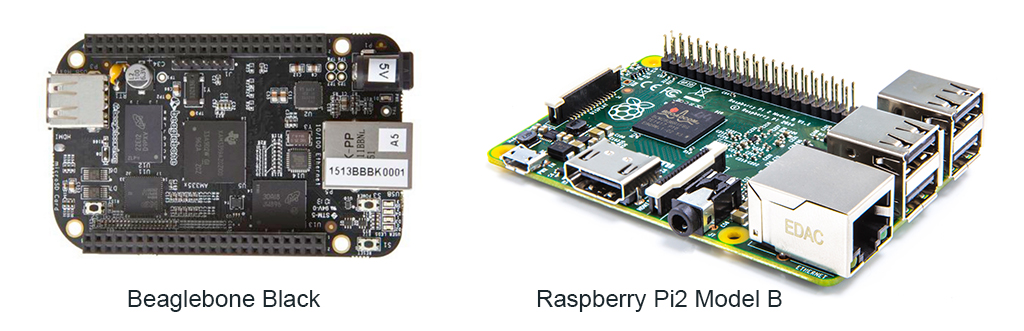
\includegraphics[width=0.7\linewidth]{picture/commodityhardware.jpg}
\caption{Beaglebone Black and Raspberry Pi2 Model B}
\label{fig:commodityhardware}
\end{figure}

\subsection{Similar Solution}
\subsubsection{FPGA accelerated market data feed}
Engineers are not satisfied with the traditional CPU based acceleration solution, and developed an alternative hardware architecture that solves the problem of buffering and filtering high frequency data. This solution introduces direct connection between FPGA chip and network interfaces, the Celoxica AMDC board enables dual feeds for single chip. Compressors and filtering program are burned in the FPGA\cite{morris2009fpga}. The acceleration of stream processing in this solution lies in the customized hardware algorithm in FPGA, and data streams goes directly to the RAM of user cores via DMA message tunnel, the IO frequency of which is higher than that in network interfaces, the structure is shown in picture \ref{fig:4}.\\
\begin{figure}[htbp]
	\centering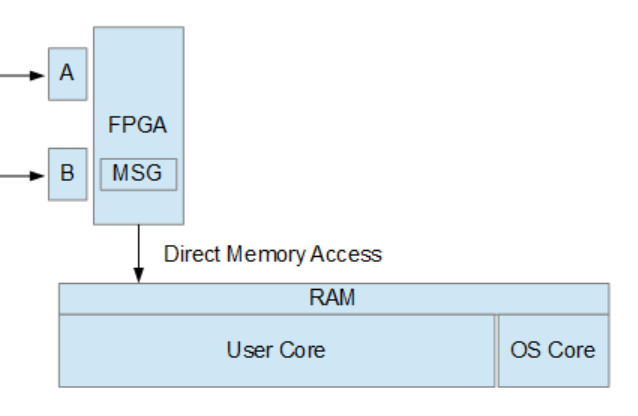
\includegraphics[width=3.5in]{picture/FPGAcall.png}
	\caption{Overview of A-B streaming infrastructure}
	\label{fig:4}
\end{figure}\\
However, this solution requires high investments in hardware, especially the motherboard and printed FPGA. Scalability is another weakness of this solution, it does not provide easy solutions for large scale implementations, especially in the scenario of bandwidth upgrading from 1Gb to 10Gb Ethernet. The NIC chip and interfaces need to be redesigned and reimplemented in the printed FPGA chip, and against the principle of System On a Chip, that the algorithm and application should be maintained only by the system supported by the hardware, not the hardware itself\cite{klaas2004system}.\\
\subsubsection{TH Express interconnection network}
TH Express interconnection network is the local area net framework for the Chinese Galaxy series super computers. It is a fat-tree topology network, and consisted of two main parts: communication network and monitor/diagnose network\cite{yang2011tianhe}. The former one connects computational nodes, the latter one checks machine status and resolves runtime error.The researchers developed a scalable network interface hardware High-Radix Routing Chip, and using RDMA method to access multiple memory spaces with unified offset, reducing processing time, improve the scalability and increasing the potential bandwidth. The architecture is shown in the picture \ref{fig:tianhe1a}\\
\begin{figure}
	\centering
	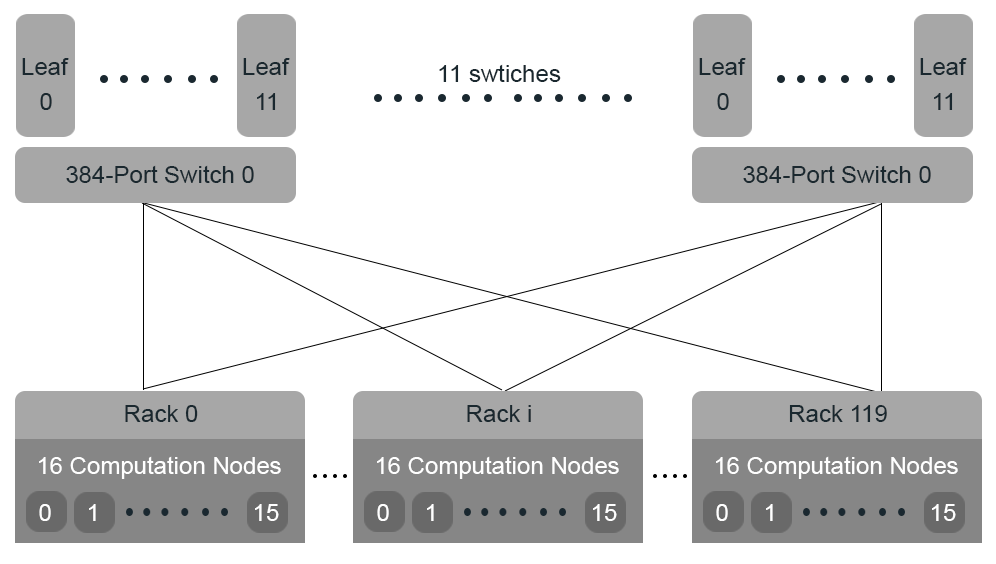
\includegraphics[width=0.7\linewidth]{picture/tianhe1A.PNG}
	\caption{Tianhe 1A interconnection network architecture}
	\label{fig:tianhe1a}
\end{figure}
Solution provided by TH Express is efficient but too expensive to achieve, however, it provides an approach to reduce latency in high frequency network data supporting the massive parallel processing system, that scalable commodity hardware supported by RDMA can improve the reliability and bandwidth of the network.\\
\subsubsection{Enyx`s ARM-based System On a Chip solution}
Market data hardware infrastructure providers offer variates of solutions to reduce the latency in market data feed. The most recent solution is to implementing FPGA hardware algorithm with ARM based SoC. It accepts A-B feed from normal network interfaces and perform the decompression and filtering via algorithm in FPGA, the ARM CPU focuses on mission dispatch and status monitor.\\
One of the well-known solution provider is the Enyx, the platform of which is based on Altera Stratix V FPGA board. The rebroadcasting latency for the FPGA supported market data processor can reach 1050 nano seconds, and average latency is 1300 nano seconds\cite{ciscoWhitePaper}. Other commercial solutions supports implementation of trading logic in the switch FPGA, that the terminals from the traders only monitors the macro status of the system, and execution of trading signals only relies on the hardware implemented applications, which reduces the event-reaction time significantly.\\ 

\chapter{Methodology}
This chapter introduces four key technology in the project: Remote direct memory access, fat-tree topology, MPI-CH, and  field-programmable gate array assisted CPU computation.\\
% Please add the following required packages to your document preamble:
% \usepackage{booktabs}
\begin{table}[H]
\centering
\caption{My caption}
\label{my-label}
\begin{tabular}{@{}l|ll@{}}
\toprule
Technology                                                               & Implementation                                                          & Details                                                                                                                                                          \\ \midrule
\begin{tabular}[c]{@{}l@{}}Remote Direct \\ Memory Access\end{tabular}   & Infiniband RMDA                                                         & \begin{tabular}[c]{@{}l@{}}Infiniband verb implementation\\ over RDMA data engine and \\ protocols\end{tabular}                                                  \\ \hline
\begin{tabular}[c]{@{}l@{}}Fat-tree topology \\ netowork\end{tabular}    & \begin{tabular}[c]{@{}l@{}}Fat-tree over\\ infiniband RDMA\end{tabular} & \begin{tabular}[c]{@{}l@{}}Fat-tree network for RDMA \\ internet layer to communicate\\ more efficiently\end{tabular}                                            \\ \hline
\begin{tabular}[c]{@{}l@{}}Message Passing\\ Interfaces\end{tabular}     & MPI-CH standard v2                                                      & \begin{tabular}[c]{@{}l@{}}Integrating the hardware platform \\ to a multi-process cluster over a \\ shared memory managed by RDMA\end{tabular}                  \\ \hline
\begin{tabular}[c]{@{}l@{}}Field Programmable\\ Field Array\end{tabular} & Sparta FPGA                                                             & \begin{tabular}[c]{@{}l@{}}Introducing FPGA to assist CPU \\ clusters handling problems that \\ are hard to be separated into \\ paralleled threads\end{tabular} \\ \bottomrule
\end{tabular}
\end{table}
The implementation of these methods are carefully selected, to fit the architecture and achieve the best performance. MPI structure with RDMA is not a new technology, however, it has not been implemented over the dual-feed switches yet, so the design of the structure is different from a normal MPI cluster. The network topology in implementation is also another innovation because this design is usually in the computational nodes, and the project introduces fat-tree RDMA network to reduce the requirement in hardware performances of single node.\\
\section{Remote Direct Memory Access(RDMA)}
The introduction of remote direct memory access technology is inspired by the architecture design in TH Express high performance interconnection network switches, which implements the RDMA as a basic memory space management infrastructure to enable the scalability of the system using distributed cluster as an virtual switch rather than using customized central switch. The basic principle of using RDMA is to trade for efficiency with the cost of memory space and bandwidth within the switch system.\\ 
Remote direct memory access technology is developed over the traditional Direct Memory Access engine, filling the requirement of encapsulating details in data copying and shifting in cloud platforms\cite{archer2012remote}. The technology enables developers ignoring the implementation in data transmission among computation nodes, and focusing on the design of the parallel computing algorithms themselves. The actual RDMA protocol family is consisted of three protocols:
\begin{itemize}
	\item Remote Direct Memory Protocol
	\item Direct Data Placement Protocol
	\item Maker UDP Aligned
\end{itemize}
The protocol family focuses on providing data availability over the interconnected networks without operating system kernel involved, and direct data exchange in the network interfaces. The technology requires no additional buffering spaces and performs under atomic operations: read/write, send/receive\cite{RobertRDMAintro}. \\
The problem of supporting remote direct memory access is the implementation of user-level data access over traditional network protocols, which would inevitably require the interception from system kernel model\cite{liu2004high}. Remote DMA requires interception before data swapping and access in the physical memory, therefore interception in kernel model must be implemented. However, the feature required by applications that RDMA should hide the details of data shifting and other system-level details, and application structures should not be infected by the implementation. For example, data shifting within the multi-processing distribution system should not infect the processes of single threads, which may require virtual data blocks whose actual address is on the remote node. Another common scenario is the asynchronous exiting sequence of different threads, which requires asynchronous data shifting in entering and existing actual memory spaces. \\
Engineers have introduced several features in the implementation of RDMA protocols, that bypasses the kernel model in the traditional internet protocol layers, and created a virtual tunnel among buffers in the threads running on separate nodes in the cluster.\\
RDMA plays as a core part in the project, which enables the open sourced hardware performs integrated computation with incoming data feeds and share without CPU involvement,  minimizing the computational power cost by increasing the bandwidth and memory space cost, which is far easier and cheaper to achieve than high performance processors.\\
\subsection{Two Important Concepts: Verbs and Queue Pairs}
The implementation of verbs and queue pairs enables the RDMA performing kernel bypassing and CPU-free message handling. The verbs are abstract APIs that can be called in the application layer indicates that the application is implementing RDMA thus the layers below, especially the traditional socket-based internet protocol layers will be covered and the network interface card should be ready to be turned into remote memory direct access enabled model,  which will handle UDP packages with DDPP header different from other packages that it will be processed by the NIC card and sent to local memory directly with RDM protocol management. The queue pairs can be viewed as the schedule handler that performing memory registry and calling the RDMA enabled NIC, or the host channel adapter(HCA) to caring pinning of the memory packages. The basic model overview is shown in picture \ref{fig:rnic}\\
\begin{figure}[H]
	\centering
    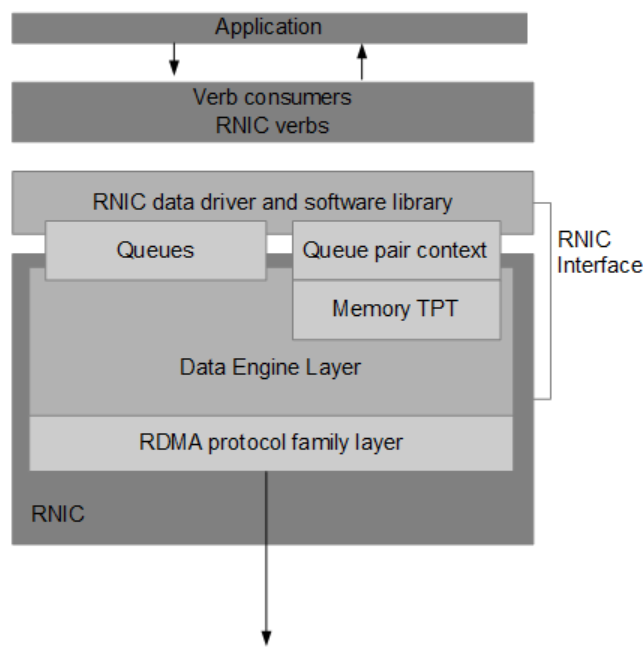
\includegraphics[width=0.4\linewidth]{picture/rnic.PNG}
    \caption{RNIC Model Overview}
    \label{fig:rnic}
\end{figure}
\subsection{Queue Pair}
The queue pair model is based on the consumer-provider model, which handling queuing of the tasks in an asynchronous way, and implements the actual data models in the network interface level to support the verb functions. The queue pair solves the problems of:
\begin{itemize}
\item Asynchronous arrival of data blocks in the interconnected network
\item Fault detection in data transmission
\end{itemize}
The queue pair is an integrated system of software, hardware and framework in remote network interface card(RNIC), and the implementation of RMDA protocol family is in the RNIC framework. The protocol family can be divided into three levels: the \(l2\) level Ethernet access mechanism implementation; the \(l3\) level IP protocol layer implementation, including IPv4, IPv6 and IPSec; the \(l4\) level protocols for TOE over TCP protocols, and RMDA protocol family including RDMA, DDP and MPA\cite{arndt2003infiniband}. RNIC infrastructure enables TCP transport support for TCP packages bypassing system kernels, which intercepts data exchange from NIC to memory. \\ 
\begin{figure}[H]
	\centering
    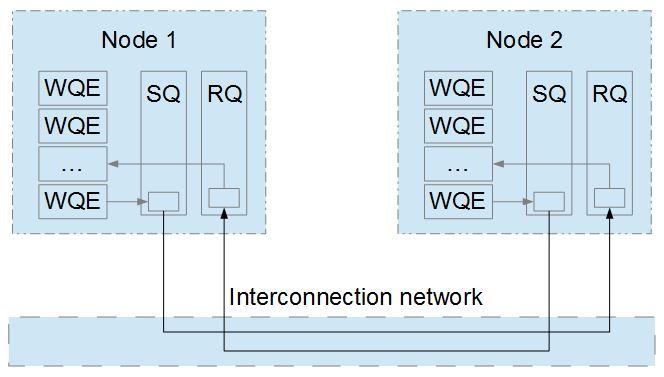
\includegraphics[width=0.6\linewidth]{picture/queuepair.JPG}
    \caption{Queued pair communication over internet}
    \label{fig:queuedpair}
\end{figure}
\subsection{RNIC Verbs}
The RNIC verbs describes the behaviour of RNIC infrastructure, and creating programming interfaces for applications to make use of the infrastructures\cite{hilland2003rdma}.  The RDMA is built upon a consumer-provider model, and the verb methods act as the middle ware between the application consumers and actual queuing pairs inside the RNIC software logics.\\ 
The verb specifications defines functions and semantics the application need to access the RDMA protocol layers, however, the verbs only include connection management and tear-down semantics, and availability to additional protocol layers  are not defined in the verbs.\\ 
\subsection{Implementation Details of Verbs}
The implementation of RNIC verbs are related to the actual policy defined by the queue pair politics, and different in actual infrastructure environment. In this project, the RDMA is the memory accessing system which provides buffering services for dynamic hardware structure for high performance system. \\
\subsubsection{Memory management}
RNIC introduces two concepts in memory management: memory window and queued pairs. The memory window manages the organization of contents in each node, and queued pairs defines the way separate nodes communicating with each other.\\
The memory windows are the basic swap element between the actual memory block and RNIC buffer\cite{garcia2006binding}. The RDMA introduces memory windows mechanism to perform memory registration and management. The remote memory shifting and offset table management are implemented through memory windows. \\
Memory space management are performed through RNIC data drivers via Tagged Offset\cite{boyd2007memory}. From the application consumer view, the memory spaces are continuous and the application can visit the entire 'shared' space by applying simple offset, but it works different from the queue pair view.\\
The queue pair is the mechanism which work requests are translated by the verbs into the interfaces provided by RNIC library, and be ready to enter the implementation of the data engine before going into the actual internet protocols. The working queues are maintained by separate nodes, and perform as the basic element of content swapping instructions. The swapping of the memory content, instructed by working queue I/O, is managed by STag access control:
\begin{lstlisting}[breaklines,breakatwhitespace,caption={STag access control},label=stag-psudoCode]
swapContentViaRNIC(QueuedProcessID qpid){
	MemoryPointer mwPointer = getLocalMemoryWindowByQPID(qpid);
	MemoryPointer mwDestiPointer = getDestiMemoryWindowByQPID(qpid);
	//Get the destination from queued pair
	ReceiveQueue rq = getReceiveQueueID(qpid);	 
	try{
		//Pop qpid from the send queue
		SendWorkingQueue.pop();				
		SwapMemory(mwPointer, mwDestiPointer);
	}catch(WorkingQueueNullException e){
		e.printStackTrace();
	}catch(MemoryException e){
		e.printStackTrace();
	}
	//Push the qpid into the receive queue
	re.push(qpid);								
}
\end{lstlisting}
So the problem lies in the strategy in choosing the strategy in the cross-node STag management. We can choose either using the same queued process id for all queued pairs, and client can seamlessly access the process registered with the same id in the server, or using different process id on each queued pairs, and managed by the client-server communication.\\
Both ways have problem: for the first solution, multiple clients can access each other`s process for they enjoy the same id in the server, which is public accessible; the second solution cannot fulfil the requirement of unified memory window management in multi-client environment, which servers need register multiple memory windows for separate clients.\\
The solution provided by RNIC is a combination of both solution:
\begin{itemize}
	\item At binding phase: queued pair id binds with each memory window, and different in separate nodes;
    \item At accessing phase: memory window with QPID is registered in both source and destination paired queues with same QPID;
\end{itemize}
\section{Fat-tree topology implementation over RDMA}
\subsection{Reducing the Cost in Node Intercommunication}
Cost in node intercommunication lies in to aspects: the content transmission speed between the network interfaces and memory spaces, and the latency in data links among nodes.\\
Data swapping within RDMA system is a bandwidth consuming performance, and the efficiency in data transformation is the threshold for the overall efficiency of the system. \\
In the data engine level, NIC can access the data blocks with the direct memory addresses without CPU, and improving the accessing speed of data by direct I/O performances from NIC to memory. 
\begin{lstlisting}[breaklines,breakatwhitespace,caption={Direct Data access from NIC to memory},label=nic-psudoCode]
SwapMemory(Memorypointer source, Memorypointer destination){
	//The pid in different client is different
	QueuedProcessID destiPID = receiveQueue.pop().getPID;
	Memorypointer desti = 
		destination + getOffset(source, destination);
	try{
		kernel.directWriteToMemory(desti,destiPID.getContent());
	}catch(MemoryIOException e){
		e.printStackTrace();
	}  
}
\end{lstlisting}
In the network topology level, the RDMA network protocols introduces fat-tree topology, which 'parent' nodes have the bandwidth aggregating bandwidth of all children nodes, and the perfect shifting mechanism guarantees the minimum cost in data shifting.\\
The implementation of perfect shifting is based on one assumption: most of instructions performed by applications require data from adjacent memory blocks $T_{i+1}(d)=Addr_{i}+V(T_{i}(d))$, therefore, the 'next step' data requirement process always requiring data either:
\begin{itemize}
	\item Require data from local memory space
    \item Require data from the neighbour nodes with the same parents
\end{itemize}
The implementation of dual feeds in data sources also reduces the time cost significantly, for the bypassing of kernel model in UDP package processing, the client in the network interface in switches works different in error processing, and node level error can be detected in leaf level switch. Comparing to flat structured centralized switch, the fat-tree topology interconnection reduces the expected error detection time from $E(T_{t}|e)=E(T_{node}|e)+E(T_{route})$, however, the expected time of processing error in node($T_(node)$) is a constant, assuming the cluster is homogeneous, and reducing the error processing time in network transmission phase.\\
\subsection{Analysing flat topology and fat-tree topology}
\begin{figure}[H]
	\centering
    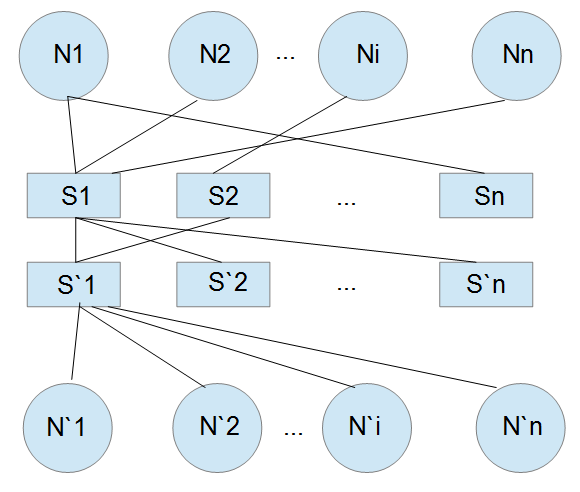
\includegraphics[width=0.4\linewidth]{picture/FlatStruct.PNG}
    \caption{Flat structured network}
    \label{fig:flat}
\end{figure}
The nodes can be divided into three groups according to the topology position to each other:
\begin{itemize}
	\item Adjacent nodes: nodes have the same parent hub
    \item Non-adjacent nodes in the same field: nodes have different parent hubs, but the hubs have direct interconnection
    \item Non-adjacent nodes in different field: nodes have different parent hubs, and the hubs have no direct interconnection
\end{itemize}
As shown in picture \ref{fig:flat}, the $N_{i}$nodes can detect and process errors in transmission and calculation, and $S_{j}$ works as the network hub which cannot process data errors. The average processing time from node N1 to adjacent nodes in network can be divided into three parts:\\
% Please add the following required packages to your document preamble:
% \usepackage{booktabs}
\begin{table}[H]
\centering
\caption{Average processing time for node N1}
\label{tab:n1proc}
\begin{tabular}{@{}ll@{}}
\toprule
Equation                                                                                          & Comment                                       \\ \midrule
$E(T_{adj})=T_{\widehat{N_{1}S_{1}N_{i}}}=\frac{\sum_{1}^{n}T_{i}}{n}$                            & i is the adjacent node                        \\
$E(T_{\widehat{N_{1}S_{1}{S}'_{1}N_{j}}})=2\times E(T_{adj})+2\times T_{\widehat{S_{1}{S}'_{i}}}$ & j is the non-adjacent node in different field  \\
$E(T_{\widehat{N_{1}S{N}'_{k}}})=2\times E(T_{adj})+E(T_{\widehat{S_{1}{S}'_{i}}})$          & k is the non-adjacent node in the same field \\ \bottomrule
\end{tabular}
\end{table}
From the equations it is easy to observe that the most time-consume process is the error detection when data is route through different fields, however, this could be frequent even we assume that the instructions in most cases process data in the adjacent node, because the switch nodes in different nodes in the node cluster, for example, $N_{1}$ and ${N}'_{1}$ could be logically adjacent in the computational cluster it connects to.\\
There are two options to reduce data processing time in the switch cluster shown in the table \ref{tab:n1proc}, one is to make all nodes adjacent to each other, however, the structure of the centralized hub could be over-complicated, another one is to to connect all the fields together,the problem is the complexity in constructing the interconnection network. A full mapping among the field hubs requires each hub supporting bandwidth of $bandwidth_{n}\times n_{fields}$, which can be very costing if we need to implement the high bandwidth in each field node.\\
One possible solution to avoid the increment of bandwidth requirement is to implement layered interconnection network rather than a flat structure, which resolve the bandwidth requirement to the back bone layer rather than the entire communication network. \\
\begin{figure}[H]
	\centering
    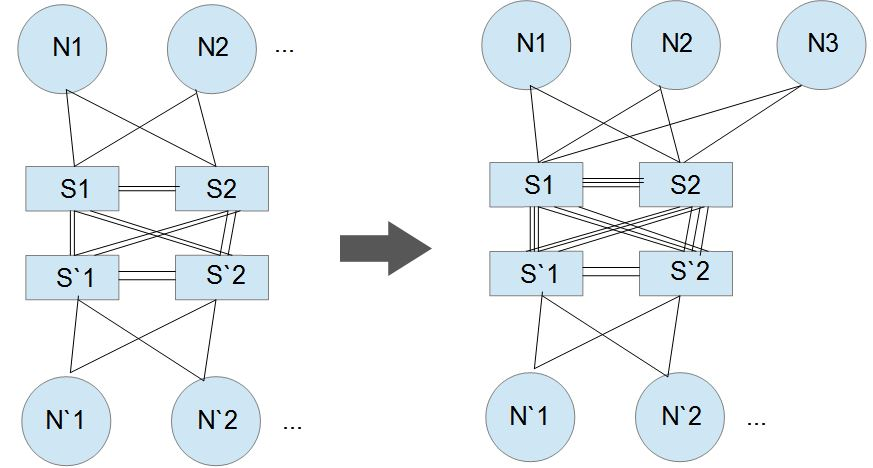
\includegraphics[width=0.6\linewidth]{picture/flat_addNode.JPG}
    \caption{Adding one node in flat mapping in the same field, six connections are changed}
    \label{fig:flatadd}
\end{figure}
The implementation of a tree-structure properly solves the problem, which not only provides a layered infrastructure which implements an aggregating bandwidth requirement from leaves to the root upstream, but also ensures the scalability of the system at the minimum cost, and the binary tree search time is $log(N)$ \cite{ellis1980concurrent}, because the increment in leaves only affects the sub-nodes in certain fields, rather than the entire system.\\
\begin{figure}[H]
	\centering
    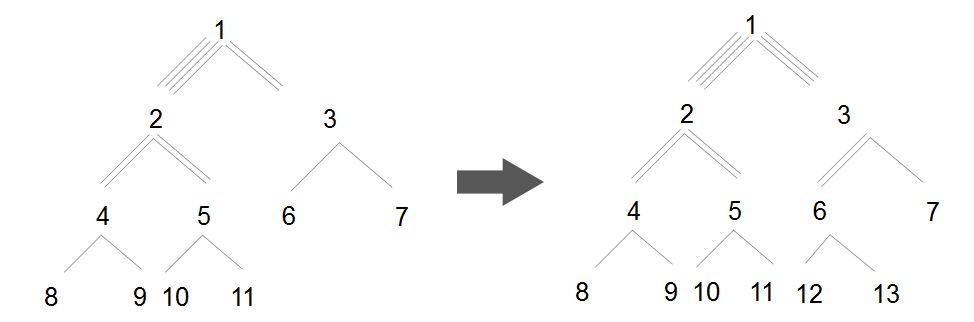
\includegraphics[width=0.6\linewidth]{picture/tree_addNodes.jpg}
    \caption{Adding nodes in tree structure, only two interconnections are changed}
    \label{fig:addnode}
\end{figure}
\subsection{Rebalancing the fat-tree over network bandwidth}
Another benefit of introducing the tree topology is the quick rebalancing feature of a tree topology network. The unbalanced tree will cause an unbalanced bandwidth load in the system. Advanced algorithm can rebalance the tree from a vine to a balanced binary tree with the time complexity of$O(n)$, and the amount of the nodes only have linear affect on the rebalancing practises. The extreme situation is a $m$ depth vine, whose root only have one leaf in one side, and another vine with $m-1$ depth vine.\\  
First, introducing the compressing of a vine in the rebalancing:
\begin{lstlisting}[breaklines,breakatwhitespace,caption={Direct Data access from NIC to memory},label=compression-psudoCode]
compression(NodePtr root, Integer count){
	NodePtr scanner;
	NodePtr child;
	Integer i;
	scanner = root;
	for i from 1 to count{
		child = scanner.right;
		scanner.right = child.right;
		child.right = scanner.left;
		scanner.left = child;
    }
}
\end{lstlisting}
and the steps from $k$th compression to $(k+1)$th compression can be shown as the figure below:
\begin{figure}[H]
	\centering
    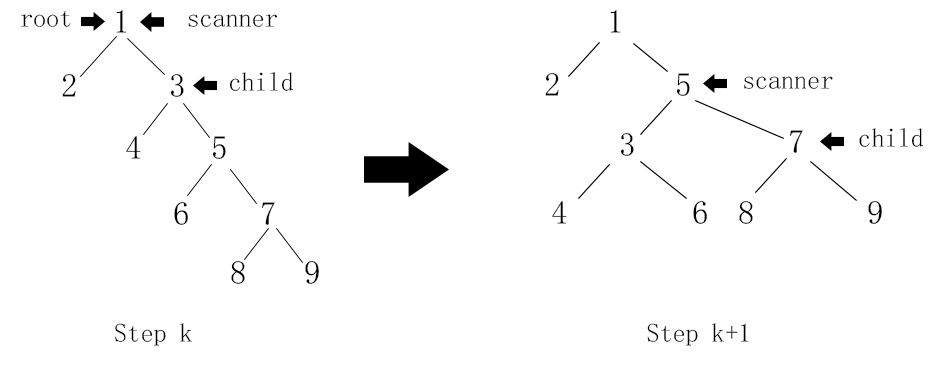
\includegraphics[width=0.6\linewidth]{picture/compression.JPG}
    \caption{Compression step k to step k+1}
    \label{fig:compression}
\end{figure}
The compression process will be performed each turn in rebalancing, for an vine with $n$ depth, each step will make a compression of the rest $\frac{n}{2}$ branches, and the node of the vine can be a complete binary tree, take the example showed in picture \ref{fig:compression}, nodes 2,4,6,8,9 are all complete binary trees, and the compression will not change the structure of the binary threes, because the only the vine nodes 1,3,5,7 are changed by the compression process\cite{stout1986tree}.\\
The rebalancing of the tree structure resolves the balancing problem of interconnection bandwidth, take the bandwidth requirement of node 5 for example: in step k before rebalancing, the bandwidth requirement of node 5 on the left side is $b_{1}$ for only one node, and on the right side is $\sum_{m}b_{i}+1$, $m$ is the amount of the leaves after vine node 5. After rebalancing, the bandwidth of node 5 on each side is the same($2\times B_{b}$, $B_{b}$ is the bandwidth of a balanced tree).\\ 
The introduction of rebalancing tree in the network topology of fat tree is for the stable scalability, and new nodes adding to the system will not have to be added following certain topology rules: the balancing of bandwidth requirement are maintained by the master node automatically, and the topology of the system is maintained dynamically.\\
\section{RDMA verb implementation: Infiniband Verbs}
Infiniband verbs, or the iverbs, are the verbs supported by infiniband RDMA protocol family which supports the implementation of RDMA over general hardware clusters. The build-in network topology management can be configured into fat-tree, which is discussed above that we want to introduce in the system. \\
The Infiniband provides upper-layer protocols(ULPs) supporting not only RDMA itself, but also most features in MPIs. The reason not using the entire Infiniband protocol family is that the support of message passing interfaces in infiniband is ill-supported in scalability, and the version we use for multi-processor interface for the open-source hardware cannot perform ideally in the infiniband pre-configuration, because the passing interfaces designed in the iverb is for much heavier use, including distributed service providers and computation. Our system is a pure message passing system which only filtering and passing message for the clusters, rather than perform the computation for them.\\
The iverb implementation can be divided into two parts\cite{bedeir2010building}. The client part and the server part. Server side mainly listens to the sockets, and react to the sockets send from the client side. The client send sockets to the servers in order to fetch data from memory directly via RDMA mechanism.\\ 
The iverbs lie in the client side when the application need to communicate with the server(the details are hidden by the verbs) to fetch data and instructions, and the server side when request are queued in the memory spaces, verbs will translate the queues to working queue elements and find the memory windows it points to, reply with the correct memory space addresses to the client to fetch the data.\\
Two features must be guaranteed for the full functioning of iverb system:
\begin{itemize}
	\item Asynchronous reliable communication: both sides will receive hanging notifications and instructions 
    \item No buffers in application level: the synchronization of the send-receive system requires no buffering especially in application memory spaces, which will cause serious problems if the content of application data is modified after sending without completing.
\end{itemize}
\subsection{Building the Passive Side}
The passive side creates and maintains an event handler for queue pairs and an event listener running in the background of network interfaces, which listens to the events from the active sides and send request queues to the queue pairs in the queue event handler directly without implementation of CPU. The iverbs in the event handler will then send the response including the memory content to lower-level protocols to be packaged into sockets, and the network interfaces will then send the package to the destinations.\\
\begin{figure}[H]
	\centering
    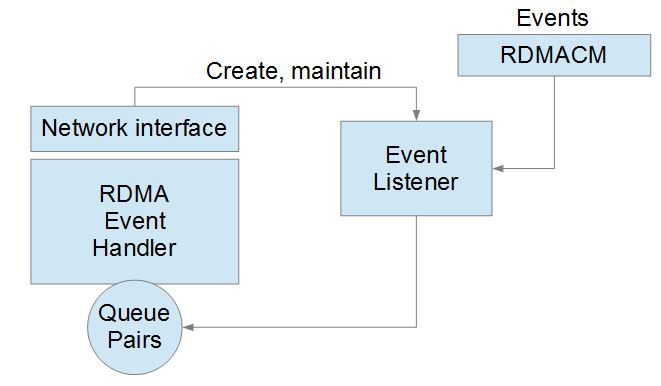
\includegraphics[width=0.6\linewidth]{picture/passive.JPG}
    \caption{Passive side design}
    \label{fig:passive}
\end{figure}
\subsubsection{Building the Active Side}
The active side runs in the client, which directly queries the content from the 'virtual' memory spaces, which is managed by the server. The active side runs a queued event handler which consumes working queue elements translated by the iverbs from the applications, and resolves receiving queues from the server, getting the actual content of the shared memory spaces.\\
The active side maintains a route to peer nodes for both active and passive sides, in order to communicate among the clusters for swapping data and instructions.\\
\begin{figure}
	\centering
    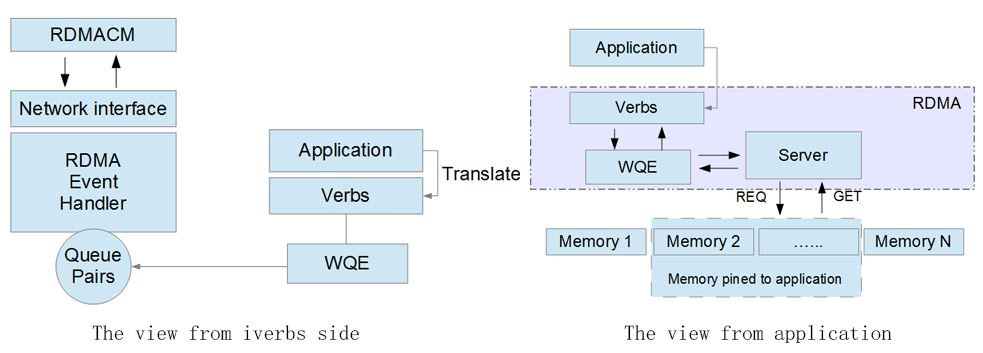
\includegraphics[width=0.8\linewidth]{picture/active.JPG}
    \caption{Active side design}
    \label{fig:active}
\end{figure}
\subsection{Conclusion}
This section introduces the RDMA method for memory management, and the fat-tree topology we need to implemented assisting the RDMA for better performances.\\
The purpose of implementing RDMA in the project is to overcome the weakness in computational power in open-source hardware, which is usually based on ARM processors with limited memory spaces. The established commercial solution to this problem usually contains an unified memory flash.The RDMA enables us to introduce fragmented memory hardware into an virtually unified one. \\
The purpose of implementing fat-tree topology is inspired by the TH-Express high performance computation clusters, which uses fat-tree interconnection network to solve the problem of low-latency network infrastructure\cite{pang2014th}. In this particular project, fragmented nodes makes it different than implementing a centralized routing system, which have fixed bandwidth balance. The implementation of rebalancing load among node clusters makes it possible to dynamically add/remove nodes.\\
\newpage
\section{MPI-CH}
Researchers introduce the MPI to build a portable and scalable multi-threading platform over heterogeneous hardware environment\cite{dongarra1995introduction}.To understand the necessity of this interface, a brief introduction of message passing model need to be introduced.\\
Most parallel applications were for scientific purposes\cite{kendall_2016}. Most of the libraries for such applications uses a message passing model for exchanging data among different cores of the machine, and normally a master manages multiple slaves by dispatching tasks and gather results.\\
The MPI-CH is an implementation of the message passing interface standard, and is widely used over multi-processing machines as a data exchange model over multiple processors performing multi-threading computations. It covers almost every aspect of MPI standards, and widely supports far more different hardware architectures compared to another well-known implementation, the OpenMPI.\\
\subsection{Introduction to SPMD and MPMD}
A parallel application can be divided into two different kinds according to the way it uses data and instructions, Single Program Multiple Data and Multiple Program Multiple Data.\\
Before introducing the SPMD and MPMD,it is necessary to make a brief introduction to the concept of Single Instruction Multiple Data(SIMD) and Multiple Instruction Multiple Data(MIMD).\\
SIMD is the model that each node execute same machine instructions over different data, for example, for array ${A}$, executing $A_{i}+1$ on each element of ${A}$ can be performed by a SIMD process by implementing the ${plus 1}$ method on each paralleled cores. MIMD works in a different way: for calculation of equation $A+B+C-D+E\times F$ , an MIMD implementation can divide the calculation into $(A+B)_{node1}+(C-D)_{node2}+(E\times F)_{node3}$ to three nodes with different instructions.
Both SPMD and MPMD are the subsets of MIMD\cite{darema2001spmd}. In this project, MPI-CH library supports both SPMD and MPMD mode, the system can differ the model by using the command line tool indicating how the program and data being seprated.\\
\subsubsection{Single Program Multiple Data}
Single Program Multiple Data(SPMD) is the parallel application which only implements one application, and execute it among each node with different sets of data.\\
A good example of message passing model is a shellsort process: for an $l$ length array $A_{l}$, the shellsort process divides the array into $\frac{l}{mod(\frac{l}{2})}$ fragments, and perform quicksort process on each fragment.The quick way to improve the efficiency of the algorithm is to place each quicksort process on a independent computational core, therefore, the time complexity only depends on the strategy of choosing the length of steps $mod(\frac{l}{2})$. However, it leaves a problem of communication among the cores.\\
For step $k$, the algorithm uses $n$ amount of cores, and in step $k+1$, the content in the memory space of each core will have the following two steps:
\begin{itemize}
	\item{1.} Merging together into a new array ${A}'$
    \item{2.} Dividing ${A}'$ into $\frac{n}{2}$ fragments and dispatching them to $\frac{n}{2}$ cores
\end{itemize}
Therefore, the programmer only need to design the dispatching mechanism and quicksort algorithm in each core. However, the solution could be cumbersome to achieve without MPI model due to the fact that for each step, the number of cores need to wake and perform send/receive practises will be different, and the designer need to predict the number of cores in each step. However, the time cost in communication is very high as the centralized node need to communicate to each node two times each step.\\
\subsubsection{Multiple Program Multiple Data}
Multiple Program Multiple Data performs parallel practises in a different way. Take the shellsort for example, if the parallel application is running on a heterogeneous cluster, whose node has different software and hardware structure and the programmer need to design and implement different sorting algorithm on each node. Therefore the step $k$ to $k+1$ could be:
\begin{itemize}
	\item{1.} Merging the fragments into new array ${A}'$
    \item{2.} Querying the infrastructure library and forming the dispatching strategy for step $k+1$, including the number of nodes, structure of the implemented nodes and data requirements for each node
    \item{3.} Implementing $k+1$ step, and divide the array ${A}'$ into required fragments, transmit the data into the destination
\end{itemize}
The MPMD program is hard to design due to the difficulty in managing the data fragmentation process, which differs according to the configuration of each node.\\
MPI-CH implements both SPMD and MPMD models, and the host can differs the structure by using command line to submit tasks from master to slave nodes.
\subsection{The architecture of MPI-CH}
The core part of MPI implementation is the send-receive pair between processes, forming a programming interface following certain message protocols with semantic specifications over varieties of machine implementations.\\
The architecture of MPI-CH standard can be abstracted as the picture below:
\begin{figure}[H]
\centering
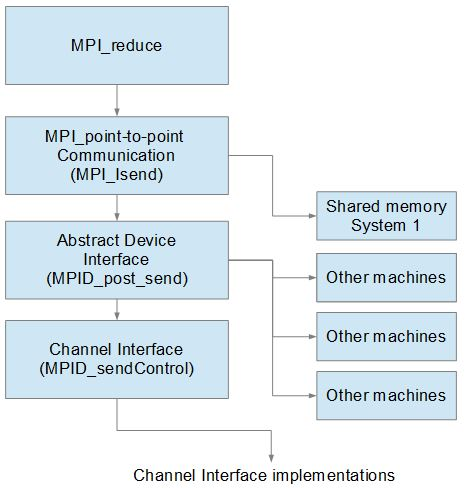
\includegraphics[width=0.6\linewidth]{picture/MPIarchitecture}
\caption{MPI architecture}
\label{fig:MPIarchitecture}
\end{figure}
The design for the MPI-CH infrastructure follows the following principles\cite{gropp1996high}:
\begin{itemize}
	\item Sharing code without compromising in performance over the actual implementation
	\item The MPI-CH should be easy to dock on different platforms with minimized amount of code changing
\end{itemize}
The first principle is to meet the need of re-implementation lower-level objects in MPI implementations over opaque objects, including communicators with tags on it, because most of these contents in MPI-CH is platform independent, and code sharing will solve the problem of dynamic scalability. The second principle requires modularised design of the infrastructure, which can replace the platform independent modules, especially the sharing part, easily and dock to the platform with minimum cost.\\
The implementation of MPICH can be split into three levels according to the sequence from application to the actual hardware.\\
\subsubsection{MPI API}
The MPI reduce, or the MPI API for the applications, are the highest layer which implements user-level abstract objects and the user applications can introduce these elements to get access to MPI-CH managed resouces.\\
The high portability feature of MPI-CH makes the interfaces easy to use and independent to actual hardware. One application can run on different MPI-CH supported hardware clusters by using configuration parameters. The entire application can be wrapped by two functions: MPI\_Init(num\_arg,*vec\_args) and MPI\_Finalize(). The program can perform both SPMD and MPMD inside the curve, and the MPI standard does not define the behaviour inside body\cite{mpich_doc}.\\  
\begin{lstlisting}[breaklines,breakatwhitespace,caption={Example of using MPICH initialization-finalization pair in C},label=compression-psudoCode]
#include<mpi.h>
int main(int argc, char** argv){
	MPI_Init(NULL, NULL);
	int processor_size;
	MPI_Comm_Size(MPI_COMM_WORLD, processor_size);
	int processor_rank;
	MPI_Comm_Rank(MPI_COMM_RANK, processor_rank);
	char processor_name[MPI_MAX_PROCESSOR_NAME];
	int name_len;
	MPI_Get_processor_name(processor_name, &name_len);
	/*-----------------/
	/ Perform algoritm /
	/-----------------*/
	 MPI_Finalize();
}
\end{lstlisting}
\subsubsection{Communication mode in MPI}
It is essential to introduce the communication mode defined in the MPI standard before moving to the actual implementation. The MPI standard defines four communication mode: \textit{Standard}, \textit{Synchronous}, \textit{Buffered} and \textit{Ready} modes\cite{dimitrov1999efficient}. It is easy to understand that RDMA always need to transfer small amount of data in high frequency over the network, therefore the protocol strategy cannot be too complex. The RDMA introduces rendezvous communication protocol to perform the transmission.\\
\begin{figure}[H]
\centering
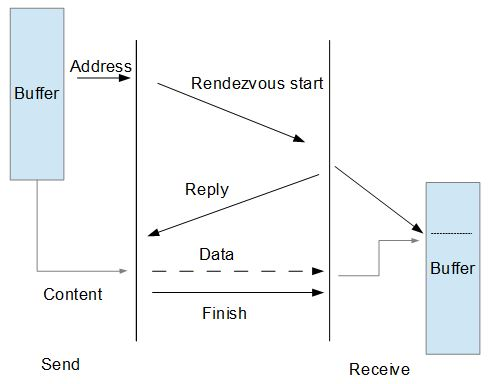
\includegraphics[width=0.6\linewidth]{picture/rendezvousMode}
\caption{Rendezvous communication in RDMA}
\label{fig:rendezvousMode}
\end{figure}
This zero-copy rendezvous protocol in RDMA works in the following sequence:
\begin{itemize}
	\item[1.] The buffer address is wrapped into control messages and transmitted to the receiver
	\item[2.] The receiver decodes control message and find the address in the receiver`s buffer, and send acknowledge message to the sender
	\item[3.] The sender sends data to receiver, and send finish segment when the transmission is finished
\end{itemize}
It uses eager strategy in pushing data to the receiver, however, there are still problems in this send-receiver strategy, especially when MPI implements the RDMA feature. The problem will be discussed afterwards.
\subsubsection{Abstract Device Interface}
The MPI-CH implements the mechanism Abstract Device Interface(ADI) in order to provide abstract services for the upper level functions, and hide the details of hardware implementations to the applications\cite{gropp1994abstract}. The message passing happens in this layer when the application uses MPI\_send or MPI\_receive, which indexed by the \textit{handle}, and queued in a way to ensure the execution sequence. The queue is managed by the MPI-CH directly and abstracted from the hardware implementation, and the handlers of IO behaviours are invoked by the lower layer, which slurp the contents and package them into proper format to suit the requirement of different mediums. The descriptions in handlers defines the type of interfaces it needs to be invoked.\\
The idea for the ADI design is to abstract the communications among nodes, and parallel scheduled from the view of applications should have no difference between local cores and remote ones. This due to the fact that MPI standard defines only the local performances in the first version of standard, and the development in network technology enables the hardware designer to introduce remote resources into a bundled parallel computing structure\cite{liu2004high}. 
ADI contains three queues: \textit{send\_queue}, \textit{posted\_recv} and \textit{unexpected\_recv}.
Send queue is for the outgoing messages, and the other two are for receiving messages. The reason for dual queues for receiving is for the asynchronous communication. Application can have the two scenarios when receiving the message from other nodes in MPICH:
\begin{itemize}
	\item The application is ready for receiving a message, and send \textit{MPI\_recv} request to the ADI layer via the API
	\item The application is not ready for any new messages, however the ADI layer receives a message with the handler pointing at this node
\end{itemize}
The first one will trigger an content shift from the queue manager to the application buffer with required contents in the queue, and the second one will register a description in the MPICH runtime manager, which enables that when the application calls for the content from receiving queue it can be shifted to the user buffer directly. \\
Another queue the ADI manages is the device ranking queue, and this queue is initialized by the user when the distributed application is deployed. It contains all the devices the MPICH runtime manager have access to, and abstract the invoker as an communication interface. The application do not need to know the existence of this list, and by invoking the communication interface, runtime manager will post the messages according to the pre-configured ranking list after an outgoing handler is created. When receiving the queue, runtime system will fairly threat all the resources, and no priority in receiving queues. The ADI uses an round-robin style of circulating query around the devices and asks if there is a new message\cite{protopopov2001multithreaded}.\\

\subsubsection{RDMA channel implementated on ADI3}
MPICH introduces ADI3, the Abstract Device Interface version three, which enables programmers to implement their own communication strategy among nodes. The structure of ADI is consisted of two parts, and can be presented in the following fashion:
\begin{figure}[H]
\centering
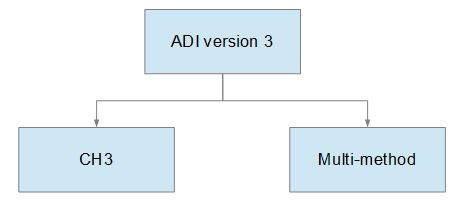
\includegraphics[width=0.5\linewidth]{picture/ADI3}
\caption{Structure of ADI3}
\label{fig:ADI3}
\end{figure}
The CH3 is a bundle of functions which implements the interfaces for different format of communications, including TCP socket and SHEMEM channel. The reason to abstract these interfaces in a subclass of ADI3 is that the CH3 bundles them into \textit{channels}\cite{mpich_doc_adi3}. The channels are based on normal Unix based socket, and introduces features such as queuing and listeners to achieve better performances.\\
The implementation of RDMA over MPI-CH structure is introduced via this mechanism, because the ADI is consisted of a set of macros and functions which allows varieties of different software-hardware infrastructure to be implemented. The design of this mechanism allows the connected hardware to implement their own message queues and data processors, which is required by the RDMA verb mechanism which overrides the kernel model in UDP socket processing and memory management by introducing its own network data exchange protocols. The RDMA channel only contains five functions, and will be discussed in the next subsection.\\
\subsubsection{RDMA channel implementation}
RDMA channel is designed for global memory share mechanism. It contains two functions for communication, \textit{put} and \textit{get}. Other three functions are for process management. Shown in the discussion of RDMA above, it maintains a queue between two nodes separately.\\
Both \textit{get} and \textit{put} are non-blocking, and the data they manipulate can go directly into the queue rather than wait until the entire process to finish. It is easy to see that the actual implementation of these two functions are different from RDMA standard description, whose communication methods are one-sided, but the actual implementation in CH3 is two-sided.\\
\begin{figure}[H]
	\centering
	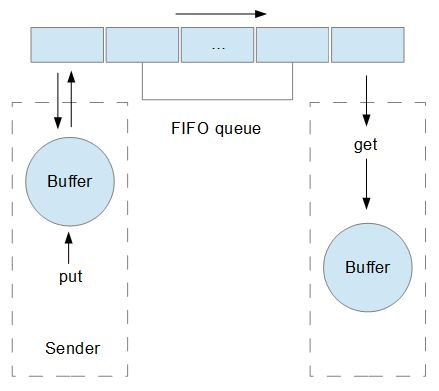
\includegraphics[width=0.5\linewidth]{picture/senderreceiver}
	\caption{The message queue between nodes}
	\label{fig:senderreceiver}
\end{figure}

\chapter{System Design and Implementation}
\section{Logical design}
\dots how I design the system: dual feed processed by ARM cpu, reconstruction and filtering by FPGA 
\subsection{Implementation of fat-tree strategy}
\section{Algorithm design}
\dots design of the thread dispatching, event sensor in the master board

\chapter{Requirements}
\chapter{Implementation and Testing}
This is the chapter in which you review the implementation and testing
decisions and issues, and critique these processes.

Code can be output inline using \verb@\lstinline|some code|@.  For example,
this code is inline: \lstinline|public static int example = 0;|  (I have
used the character \verb@|@ as a delimiter, but any non-reserved character
not in the code text can be used.)

Code snippets can be output using the \verb|\begin{lstlisting} ... \end{lstlisting}|
environment with the code given in the environment.  For
example, consider listing \ref{Example-Code}, below.

\begin{lstlisting}[breaklines,breakatwhitespace,caption={Example code},label=Example-Code]
public static void main() {

  System.out.println("Hello World");

}
\end{lstlisting}

Code listings are produced using the package ``Listings''.  This has many
useful options, so have a look at the package documentation for further
ideas.


\chapter{Results}
This is the chapter in which you review the outcomes, and
critique the outcomes process.  You may include user evaluation here
too.


%%
%% Now we are back to the standard project contents that you should include
%%

\chapter{Conclusions}
%% Uncomment this to include a separate tex file wih the conclusion contents
%\include{conclusion.tex}

This is the chapter in which you review the major achievements in the
light of your original objectives, critique the process, critique your
own learning and identify possible future work.


\bibliography{ExampleBibFile}


\appendix

%%
%% Use the appendix for major chunks of detailed work, such as these. Tailor
%% these to your own requirements
%%

\chapter{Design Diagrams}

\chapter{User Documentation}

\chapter{Raw results output}

\chapter{Code}

%%
%% NOTE that for this to typeset correctly, ensure you use the pdflatex
%%      command in preference to the latex command.  If you do not have
%%      the pdflatex command, you will need to remove the landscape and
%%      multicols tags and just make do with single column listing output
%%

\begin{landscape}
\begin{multicols}{2}
\section{File: yourCodeFile.java}
\lstinputlisting[basicstyle=\scriptsize]{yourCodeFile.java}
\end{multicols}
\end{landscape}

\end{document}

%%% Local Variables:
%%% mode: latex
%%% TeX-master: t
%%% End:
